\documentclass[12pt,a4paper]{article}

% --- Encoding and math ---
\usepackage[utf8]{inputenc}
\usepackage[T1]{fontenc}
\usepackage{amsmath,amssymb,amsthm}

% --- Graphics and layout ---
\usepackage{graphicx}
\usepackage{pgfplots}
\pgfplotsset{compat=1.18}
\usepackage{geometry}
\geometry{margin=1in}
\usepackage{microtype}
\microtypesetup{protrusion=true, expansion=false}
\UseMicrotypeSet[protrusion]{basicmath}
\usepackage[strings]{underscore}

% --- Tables ---
\usepackage{booktabs}

% --- Section formatting ---
\usepackage{titlesec}

% --- Floats, spacing, paragraph style ---
\usepackage{float}
\usepackage{setspace}
\usepackage{parskip}

% --- Verbatim with wrapping ---
\usepackage{fancyvrb}
\usepackage{fvextra}   % enables breaklines + breakanywhere

% --- Numeric tables (optional) ---
\usepackage{siunitx}
\sisetup{
    table-number-alignment = center,
    table-text-alignment   = center
}

% --- Citations ---
\usepackage{natbib}

% --- Hyperlinks ---
\usepackage{hyperref}

% --- Colored boxes ---
\usepackage{tcolorbox}

% --- Input path flexibility ---
\makeatletter
\def\input@path{{./}{./tables/}{papers/Emotion-Conditioned Risk Posture in Crypto Markets/}{papers/Emotion-Conditioned Risk Posture in Crypto Markets/tables/}}
\makeatother

% --- Section numbering: treat sections as top-level (no chapters needed) ---
\setcounter{secnumdepth}{3}
\renewcommand{\thesection}{\arabic{section}}
\renewcommand{\thesubsection}{\thesection.\arabic{subsection}}
\renewcommand{\thesubsubsection}{\thesubsection.\arabic{subsubsection}}

% --- Section formatting (your style preserved) ---
\titleformat{\section}
    {\normalfont\Large\bfseries}
    {\thesection}
    {1em}
    {}

\titlespacing*{\section}
    {0pt}
    {12pt}
    {6pt}

\titleformat{\subsection}
    {\normalfont\large\bfseries}
    {\thesubsection}
    {1em}
    {}

\titlespacing*{\subsection}
    {0pt}
    {8pt}
    {4pt}

% --- Line spacing ---
\onehalfspacing

% Format abstract full page
\makeatletter
\renewenvironment{abstract}{
    \begin{center}
        {\large\bfseries \abstractname\vspace{-.5em}\vspace{0pt}}
    \end{center}
}{}

\title{Emotion-Conditioned Risk Posture in Crypto Markets\\
\large Audit-Bundled Evidence from BTC Price and Sentiment Data}

\author{John H. Cragin\\
Independent Researcher\\
john.cragin@outlook.com\\
ORCID: \href{https://orcid.org/0009-0001-5204-5732}{0009-0001-5204-5732}}

\date{\today}

\begin{document}

\maketitle

\begin{abstract}
This paper does not evaluate market prediction, trading performance, or profitability. SpiralBrain v3.0 is used strictly as a deterministic experimental instrument to isolate participation gating as a controllable variable. SpiralBrain v3.0 is used here strictly as a deterministic experimental probe, analogous to a laboratory instrument, rather than as a trading agent or deployable decision system.

This paper presents a controlled empirical demonstration that internal regulatory bias alone can deterministically alter participation decisions under identical market inputs. Using a neurosymbolic Regulatory Intelligence system (SpiralBrain v3.0) as an instrument, we evaluate discrete risk posture outputs drawn from the posture ontology (\emph{buy}, \emph{hold}, \emph{sell}), with this experiment restricting observed outcomes to \emph{buy} and \emph{hold} to isolate participation gating.

Across a 60-day Bitcoin market window constructed from real price, volume, and sentiment data, different emotional profiles produce cleanly separated posture regimes—some consistently accepting new exposure (\emph{buy}), others consistently refusing incremental exposure (\emph{hold})—despite identical inputs and inference logic. This isolates participation gating as a first-class regulatory function, independent of forecasting accuracy, optimization, or trading performance.

The contribution is methodological rather than predictive. No claims of trading alpha, profitability, or generalization are made. All quantitative claims are grounded in an audit-bundled reference run with offline verifiability, enabling falsification without access to private inference code.
\end{abstract}

\begin{tcolorbox}[colback=gray!10, colframe=gray!50, title=What This Paper Is NOT]
\textbf{This paper does not:}
\begin{itemize}
\item propose a trading strategy
\item evaluate market prediction accuracy
\item optimize returns or risk-adjusted performance
\item claim profitability or deployability
\end{itemize}

\textbf{This paper does:}
\begin{itemize}
\item isolate participation gating as a causal variable
\item demonstrate deterministic regulation under identical inputs
\item provide artifact-verifiable falsification evidence
\end{itemize}
\end{tcolorbox}

\section{Problem Statement}

Market behavior is frequently modeled as a function of ``information'' alone. In regulatory cognitive architectures, however, internal affective regulation functions as a control layer that shapes decisions under uncertainty. We ask a narrow empirical question:

\begin{quote}
Given the same real market inputs, do different emotional profiles induce different discrete risk posture outputs?
\end{quote}

We operationalize posture as a discrete decision variable in \{buy, hold, sell\}. However, this experiment implements only \emph{buy} and \emph{hold} postures to focus on participation control—\emph{sell} signals are excluded by design. We do not attempt to backtest or optimize a trading strategy.

This study evaluates a single, fully archived experimental run to establish existence and falsifiability, not statistical generality.

The goal is to demonstrate that participation gating can be isolated as a controllable variable, not to estimate its prevalence or magnitude.

This is an existence proof for emotion-conditioned participation gating, not a market modeling study.

\subsection{Scope of Posture Actions}

This study evaluates participation control rather than full trading behavior. Posture outputs are therefore interpreted solely as decisions to accept or refuse incremental market exposure (\emph{buy} vs. \emph{hold}). Active de-risking (\emph{sell}) is defined in the posture ontology but intentionally excluded from the experimental degrees of freedom, as it represents a distinct regulatory function involving exit behavior and position state. This restriction is necessary to isolate participation gating as a causal variable under identical external inputs.

\section{Experimental Instrument: SpiralBrain v3.0}

SpiralBrain v3.0 is a Python-based neurosymbolic Regulatory Intelligence system designed to study viability-first decision-making under uncertainty. SpiralBrain v3.0 implements the Regulatory Intelligence (RI) paradigm, a viability-first cognitive framework in which internal coherence and participation restraint take precedence over task optimization \cite{Cragin2026RIParadigm}. In this paper, SpiralBrain is used strictly as an \emph{experimental instrument}—analogous to a laboratory probe—rather than as a trading agent or deployable decision system.

SpiralBrain v3.0 is treated analogously to a laboratory apparatus: deterministic, instrumented, and intentionally non-adaptive during inference, so that internal regulatory state can be manipulated as an experimental variable.

The system operates locally on standard hardware and processes aligned numerical time series without online learning, parameter updates, or stochastic exploration during inference. For a fixed input dataset, repeated runs with identical configuration produce identical outputs. This determinism allows internal regulatory state to be treated as an experimental variable rather than a latent confound.

SpiralBrain decomposes decision-making into three conceptually distinct stages: (i) signal ingestion and feature alignment, (ii) internal regulatory evaluation, and (iii) discrete posture emission. In this experiment, only the internal regulatory evaluation stage is varied across profiles. Feature extraction, thresholds, inference logic, and output contracts are held constant.

Importantly, SpiralBrain is not optimized for market prediction or trading performance. Its outputs are posture decisions representing willingness or refusal to accept additional exposure under uncertainty. As such, SpiralBrain functions here as a controlled probe for studying participation gating rather than as a forecasting model.

Emotional profiles in SpiralBrain are instantiated as fixed regulatory parameter vectors that bias the system toward caution or exploration when resolving uncertainty. These profiles do not alter market inputs, learned parameters, or decision rules; they only affect how regulatory pressure is balanced internally when identical signals are evaluated. In the present study, emotional profiles are selected deliberately to test sensitivity rather than to model realistic affect distributions.

\section{Conceptual Framework (Theory)}

We treat an ``emotional profile'' as a controlled internal condition that changes the system's regulatory weighting of risk signals, without changing the external input stream. An emotional profile is instantiated by an injected \texttt{emotional\_state} parameter vector that modulates regulatory weighting. Let $x_t$ denote the aligned market input at day $t$ (fear/greed, price, volume). Let $\theta$ denote an emotional profile setting. The system emits a discrete posture $y_t \in \{\text{buy}, \text{hold}, \text{sell}\}$ and a confidence value $c_t \in [0,1]$. The confidence value $c_t$ is treated here as a system-internal certainty signal, not a calibrated probability of market correctness.

The core theoretical claim is not about market forecasting. It is about conditional decision policy:

\begin{quote}
Holding $x_{1:T}$ fixed, varying $\theta$ can change the posture sequence $y_{1:T}$.
\end{quote}

This theory implies posture differences across profiles are expected even when the input dataset is identical, because profiles instantiate different internal regulatory biases (e.g., toward caution vs exploration). This theory is falsifiable by runs in which all profiles converge to identical posture distributions under the same \texttt{market\_data\_used.json}.

To illustrate the causal structure compactly:

\[
\exists\, \theta_1, \theta_2 \text{ with } \theta_1 \neq \theta_2
\text{ such that for fixed } x_{1:T},\;
F(x_{1:T}; \theta_1) \neq F(x_{1:T}; \theta_2).
\]

\section{Hypotheses}

We state hypotheses at the level of measurable outputs in run artifacts.

\begin{itemize}
	\item \textbf{H1 (Emotion-conditioned posture separation)}: For a fixed aligned input time series, posture outputs differ across emotional profiles.
	\\
	\emph{Falsification:} if all profiles output identical posture distributions on the same \texttt{market\_data\_used.json} (e.g., all profiles selecting buy on every aligned day), H1 is false for that run.
    
	\item \textbf{H2 (Caution-biased profiles shift toward hold)}: For a fixed aligned input time series, profiles with defensive/hazard framing produce a higher \textbf{hold} count than a neutral profile.
	\\
	\emph{Operationalization (this paper):} compare \texttt{high\_hazard\_alert} and \texttt{defensive} vs \texttt{control\_neutral} on hold counts.
	\\
	\emph{Falsification:} if \(\texttt{hold(high\_hazard\_alert)} \le \\ \texttt{hold(control\_neutral)}\) and \(\texttt{hold(defensive)} \le \\ 
    \texttt{hold(control\_neutral)}\) on the same \texttt{market\_data\_used.json}, \\
    H2 is false for that run.
\end{itemize}

This paper samples deliberately extreme regulatory modes from a high-dimensional emotional space. It is a sensitivity proof, not a coverage study: clean separation under identical inputs falsifies "emotion doesn't matter" more strongly than graded effects. Intermediate emotions and nuanced modulation are future work.

These hypotheses are evaluated on a single canonized run and are not claimed to generalize beyond that run.

Extreme profiles are used deliberately to maximize separability under identical inputs, strengthening falsification power.

\section{Risk Posture as Participation Control}

In this experiment, we implement a \textbf{participation control system} that produces only \emph{buy} and \emph{hold} postures—\emph{sell} signals are intentionally excluded to focus on the decision of whether to accept additional market exposure. This design isolates participation gating as the core regulatory mechanism.

\emph{Buy} and \emph{hold} are treated as discrete \textbf{risk postures}, not trading recommendations or forecasts. A \emph{buy} posture represents willingness to engage with market exposure under uncertainty—i.e., to accept volatility in exchange for potential upside. A \emph{hold} posture represents deliberate non-participation: the system elects to remain exposed only to existing positions and declines additional risk despite available signals. Importantly, \emph{hold} is not indecision or failure to act; it is an active regulatory choice indicating that perceived hazard outweighs exploratory opportunity.

In financial practice, posture decisions govern institutional participation, not just individual trades:

\begin{itemize}
	\item \textbf{Buy}: Increase exposure (e.g., allocate capital to risk despite uncertainty).
	\item \textbf{Hold}: Refuse incremental exposure (e.g., maintain existing positions but decline new risk).
	\item \textbf{Sell}: Active de-risking (e.g., reduce exposure to cut losses) - \emph{not implemented in this experiment}.
\end{itemize}

Banks, funds, tax advisors, and compliance teams routinely \emph{hold} even when bullish—citing governance, liquidity, or regulatory thresholds. This is not indecision; it is participation control. Our experiment models this behavior: in the SpiralBrain system evaluated here, refusal to act is implemented as an explicit, auditable decision outcome.

\section{What Changes—and What Does Not—Across Emotional Profiles}

Across all profiles, the system processes the same aligned market inputs (price, volume, and sentiment) using the same feature extraction, thresholds, and inference pipeline. Emotional profiles do not alter market data, indicators, or decision rules. Instead, they modify \emph{internal regulatory weighting}—how strongly the system prioritizes hazard suppression versus exploratory engagement when evaluating identical signals. As a result, emotional regulation influences \emph{how signals are interpreted}, not \emph{which signals are observed}.

The system does not infer or react to investor psychology; it evaluates the same numerical signals under different internally defined participation thresholds.

\section{Emotion as a Regulatory Lens}

In SpiralBrain, emotional state functions as a regulatory lens that shapes how conflicting signals are resolved. When hazard pressure is elevated, negative or ambiguous signals are amplified relative to positive momentum, raising the system's internal threshold for engagement. When hazard pressure is low, opportunity signals dominate, and the system tolerates greater uncertainty before suppressing action.

Risk aversion here is not a learned preference but an explicit regulatory parameter, fixed prior to inference and held constant across all timesteps.

\section{Internal Regulation vs External Market Emotion}

The emotional state injected into the system does not represent market emotion, investor sentiment, or trader psychology. It represents an internal regulatory bias governing risk tolerance and participation thresholds.

Analogy: Market emotion is weather (external, observable). System emotion is risk policy (internal, controllable). This paper studies policy effects on decision-making, not weather forecasting.

\section{Why This Matters for Financial and Compliance Systems}

This work has implications for systems where refusal to act is intelligence:

\begin{itemize}
	\item \textbf{Participation gating}: AI can now model "hold" as governance, not failure.
	\item \textbf{Auditability of non-actions}: Regulators can verify why an AI declined risk.
	\item \textbf{Regulatory defensibility}: Compliance teams can demonstrate controlled risk tolerance.
	\item \textbf{Uncertainty governance}: Finance relies on thresholds, not just predictions.
\end{itemize}

This is not about alpha; it's about making AI behaviorally legible to human oversight.

Analogously, a tax advisor may believe an asset's appreciation will continue while still declining to realize gains due to regulatory uncertainty. The system's hold posture models this refusal as an explicit, auditable decision.

\section{Data Sources and Alignment}

Inputs are derived from:

\begin{itemize}
	\item Crypto Fear \& Greed Index API (alternative.me) \citep{AlternativeMeFNG}
	\item Bitcoin market chart (price and volume, USD) via CoinGecko \citep{CoinGeckoMarketChart}
\end{itemize}

For \href{https://github.com/jhcragin/SpiralBrain-v3.0-public/tree/main/Emotion-Conditioned%20Risk%20Posture%20in%20Crypto%20Markets/results}{market_emotion_research_20260120_201255}, the dataset spans 60 matched UTC days, from \texttt{2025-11-22} through \texttt{2026-01-20}, inclusive. The integrator matches sources by a UTC day key formatted as \texttt{YYYY-MM-DD}.

\section{Market Window Visualization}

\begin{figure}[H]
\centering
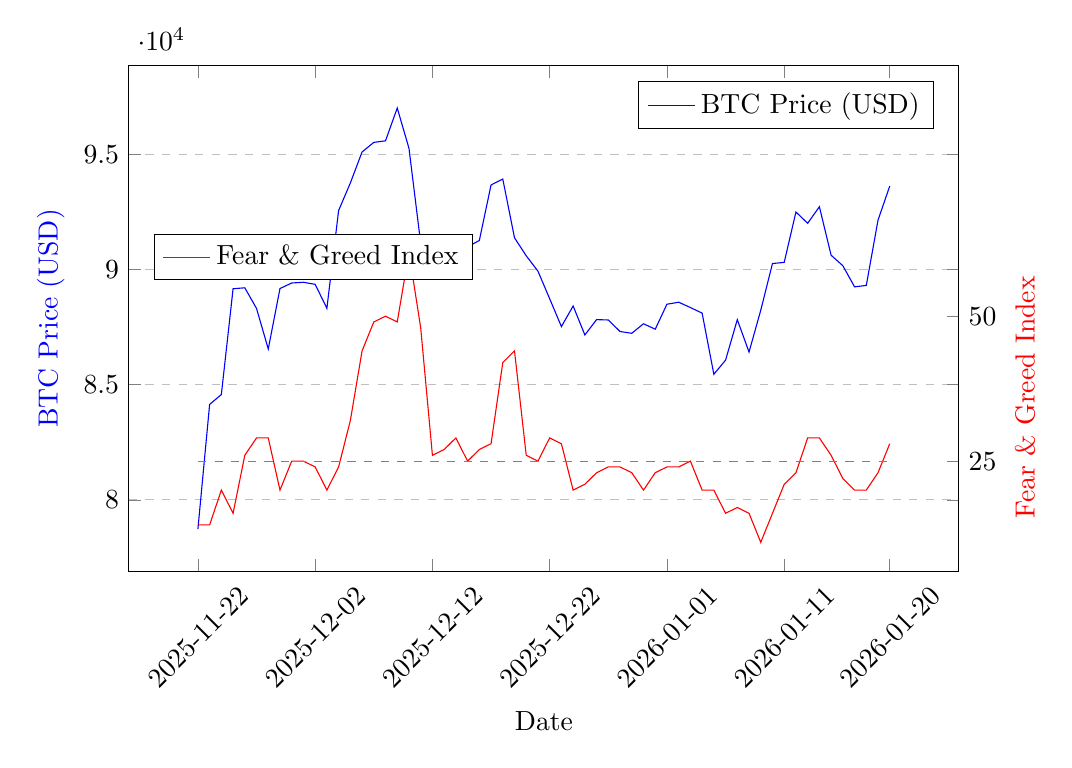
\begin{tikzpicture}
\begin{axis}[
    width=\textwidth, height=8cm,
    xlabel={Date},
    ylabel={BTC Price (USD)},
    ylabel style={color=blue},
    xtick={0,10,20,30,40,50,59},
    xticklabels={2025-11-22,2025-12-02,2025-12-12,2025-12-22,2026-01-01,2026-01-11,2026-01-20},
    xticklabel style={rotate=45},
    legend pos=north east,
    ymajorgrids=true,
    grid style=dashed,
]
\addplot[color=blue, mark=none] coordinates {
    (0, 78725.86)
    (1, 84141.78)
    (2, 84570.41)
    (3, 89162.10)
    (4, 89204.22)
    (5, 88307.86)
    (6, 86548.32)
    (7, 89170.87)
    (8, 89412.40)
    (9, 89443.40)
    (10, 89354.34)
    (11, 88312.84)
    (12, 92558.46)
    (13, 93752.71)
    (14, 95099.53)
    (15, 95516.08)
    (16, 95584.83)
    (17, 97007.78)
    (18, 95260.44)
    (19, 91134.97)
    (20, 90819.37)
    (21, 90442.02)
    (22, 90504.90)
    (23, 90983.52)
    (24, 91257.16)
    (25, 93666.86)
    (26, 93926.80)
    (27, 91373.22)
    (28, 90593.85)
    (29, 89926.28)
    (30, 88727.67)
    (31, 87520.18)
    (32, 88414.63)
    (33, 87156.56)
    (34, 87822.91)
    (35, 87807.00)
    (36, 87305.96)
    (37, 87229.78)
    (38, 87642.61)
    (39, 87406.44)
    (40, 88491.12)
    (41, 88577.42)
    (42, 88347.94)
    (43, 88103.86)
    (44, 85450.33)
    (45, 86064.95)
    (46, 87821.89)
    (47, 86413.92)
    (48, 88230.77)
    (49, 90257.43)
    (50, 90307.26)
    (51, 92494.18)
    (52, 92005.14)
    (53, 92723.21)
    (54, 90618.05)
    (55, 90162.91)
    (56, 89244.76)
    (57, 89307.09)
    (58, 92140.70)
    (59, 93619.44)
};
\addlegendentry{BTC Price (USD)}
\end{axis}
\begin{axis}[
    width=\textwidth, height=6cm,
    ylabel={Fear \& Greed Index},
    ylabel style={color=red},
    axis y line*=right,
    axis x line=none,
    ytick={0,25,50,75,100},
    yticklabels={0,25,50,75,100},
    legend pos=north west,
]
\addplot[color=red, mark=none] coordinates {
    (0, 14)
    (1, 14)
    (2, 20)
    (3, 16)
    (4, 26)
    (5, 29)
    (6, 29)
    (7, 20)
    (8, 25)
    (9, 25)
    (10, 24)
    (11, 20)
    (12, 24)
    (13, 32)
    (14, 44)
    (15, 49)
    (16, 50)
    (17, 49)
    (18, 61)
    (19, 48)
    (20, 26)
    (21, 27)
    (22, 29)
    (23, 25)
    (24, 27)
    (25, 28)
    (26, 42)
    (27, 44)
    (28, 26)
    (29, 25)
    (30, 29)
    (31, 28)
    (32, 20)
    (33, 21)
    (34, 23)
    (35, 24)
    (36, 24)
    (37, 23)
    (38, 20)
    (39, 23)
    (40, 24)
    (41, 24)
    (42, 25)
    (43, 20)
    (44, 20)
    (45, 16)
    (46, 17)
    (47, 16)
    (48, 11)
    (49, 16)
    (50, 21)
    (51, 23)
    (52, 29)
    (53, 29)
    (54, 26)
    (55, 22)
    (56, 20)
    (57, 20)
    (58, 23)
    (59, 28)
};
\addlegendentry{Fear \& Greed Index}
\draw[dashed, gray] (axis cs:0,25) -- (axis cs:59,25);
\draw[dashed, gray] (axis cs:0,75) -- (axis cs:59,75);
\end{axis}
\end{tikzpicture}
\caption{BTC Price (USD) and Fear \& Greed Index timeline for the experimental window (Nov 22, 2025 – Jan 20, 2026). Dashed lines indicate Fear/Neutral (25) and Greed (75) thresholds.}
\end{figure}

This visualization provides context for the experimental window (Nov 22, 2025 – Jan 20, 2026) by jointly displaying Bitcoin price (USD) and the Fear \& Greed Index. The period corresponds to post-correction consolidation, with sentiment transitioning from Extreme Fear toward Fear/Neutral dominance.


\section{Audit Infrastructure and Provenance}

The following sections describe the infrastructure used to support independent verification; they are not required to evaluate the empirical claim itself.

This work is designed to be verifiable offline. Each run records:

\begin{itemize}
	\item Upstream request URLs and retrieval timestamps
	\item SHA-256 hashes of raw upstream payloads
	\item Gzipped archives of raw payloads under \texttt{provenance/raw/<sha>.json.gz}
	\item The exact aligned \texttt{market\_data\_used.json} passed into the system
	\item A deterministic SHA-256 hash of \texttt{market\_data\_used.json}
\end{itemize}

For \href{https://github.com/jhcragin/SpiralBrain-v3.0-public/tree/main/Emotion-Conditioned%20Risk%20Posture%20in%20Crypto%20Markets/results}{market_emotion_research_20260120_201255}, the recorded provenance hashes are directly verifiable from the linked files.

The run metadata records the exact command-line invocation used to generate artifacts.

\section{Public Verification Package (Reviewer-Facing)}

To support journal review without requiring trust in the author or access to any private inference implementation, the offline verification materials for this paper are published at the GitHub Public Repository:
\begin{quote}
\href{https://github.com/jhcragin/SpiralBrain-v3.0-public/tree/main/Emotion-Conditioned%20Risk%20Posture%20in%20Crypto%20Markets}{Emotion-Conditioned Risk Posture in Crypto Markets}
\end{quote}

The public repository contains a frozen verification contract (\href{https://github.com/jhcragin/SpiralBrain-v3.0-public/blob/main/README.md}{README.md}), a stdlib-only offline verifier (\href{https://github.com/jhcragin/SpiralBrain-v3.0-public/blob/main/Emotion-Conditioned%20Risk%20Posture%20in%20Crypto%20Markets/verify_reference_run.py}{verify_reference_run.py}), and a canonized reference specimen under \texttt{results/}.

\section{Experimental Setup}

\subsection{System Under Test}

SpiralBrain v3.0 is treated as an instrumented regulatory cognitive system. The experiment evaluates multiple emotional profiles under an identical aligned input time series captured in \texttt{provenance/market\_data\_used.json}.


\subsection{Profiles}

The following six profiles are tested in \href{https://github.com/jhcragin/SpiralBrain-v3.0-public/tree/main/Emotion-Conditioned%20Risk%20Posture%20in%20Crypto%20Markets/results}{market_emotion_research_20260120_201255}:
\texttt{control\_neutral}, \texttt{high\_hazard\_alert}, \texttt{overconfident\_explorer}, \texttt{high\_uncertainty}, \texttt{complacent}, \texttt{defensive}.

Profiles differ only in the injected \texttt{emotional\_state} parameters (valence, arousal, hazard pressure, neuromodulator flexibility); no profile alters external inputs, feature extraction, or the output contract.

\subsection{Output Contract and Fail-Loudly Behavior}

Each prediction must emit a strict contract including posture direction and confidence. Missing required fields is treated as a hard error, causing the benchmark to fail rather than silently continuing.
\subsection{Experimental Run Structure and Interpretation}

This study evaluates a single canonized experimental run designed as an existence proof rather than a statistical estimation. A fixed, SHA-verified 60-day BTC market input series is treated as an external stimulus and passed unchanged through a deterministic regulatory system under six controlled internal conditions ("emotional profiles"). No learning, retraining, stochastic sampling, or parameter updates occur during inference. Each profile processes the identical input sequence and emits a discrete posture output per day, yielding 360 total posture decisions. The sole experimental manipulation is the injected internal regulatory bias. As such, the experiment isolates participation gating as a causal variable under identical external conditions, rather than evaluating market prediction, trading performance, or profitability.
\section{Results}

Under an identical 60-day market input series, different emotional profiles produce systematically different participation decisions. Across six profiles and 360 predictions, the system either consistently accepted new market exposure (\emph{buy}) or consistently refused incremental exposure (\emph{hold}), depending solely on internal regulatory state.

The run consists of 60 market days and 6 profiles, producing 360 predictions, all of which are valid (0 errors).

This window (Nov 22, 2025 – Jan 20, 2026) represents post-correction consolidation with Fear-to-neutral sentiment dominance, strengthening the regulatory-lens interpretation: hazard-biased profiles gated participation despite not being in full capitulation territory.

All counts in this section refer to the number of aligned days over which a given posture was selected, not to prediction correctness or performance.

In this run, emotional profiles bifurcate cleanly into two participation regimes: some profiles select \emph{buy} on every day, while others select \emph{hold} on every day, despite identical inputs.

The observed outcome is a complete separation: under identical inputs, each emotional profile selects a single posture consistently across all 60 days, with no mixed behavior.

\subsection{Confirmatory Run with Randomized Emotional Profiles}

To test whether the posture bifurcation observed in the primary experiment persists under unbiased sampling, we conducted a confirmatory run with 20 randomly generated emotional profiles. This confirmatory run is not intended to estimate frequencies, thresholds, or probabilities over emotional space, but to test whether the posture bifurcation observed in the primary experiment persists under unbiased sampling.

The confirmatory run produced 1,200 predictions (20 profiles × 60 days) with identical market inputs. Results showed the same clean bifurcation: 16 profiles produced 100\% buy signals, while 4 profiles produced 100\% hold signals, with no sell signals observed. This confirms that the buy/hold separation is not an artifact of the specific research profiles but a robust property of the regulatory mechanism.

\begin{table}[H]
\centering
\begin{tabular}{lrrrrr}
\hline
Profile & N & AvgConf & Buy & Hold & Sell \\
\hline
complacent              & 60 & 0.597 & 60 & 0  & 0 \\
control\_neutral        & 60 & 0.611 & 60 & 0  & 0 \\
defensive               & 60 & 0.547 & 0  & 60 & 0 \\
high\_hazard\_alert     & 60 & 0.559 & 0  & 60 & 0 \\
overconfident\_explorer & 60 & 0.605 & 60 & 0  & 0 \\
high\_uncertainty       & 60 & 0.601 & 60 & 0  & 0 \\
\hline
\end{tabular}
\caption{Posture selection counts across 60 aligned days under identical inputs, by emotional profile. AvgConf reflects the system's internal certainty signal for the posture actually selected (Buy or Hold), and is not intended for cross-posture comparison.}
\label{tab:posture_dist}
\end{table}

This pattern also supports H2 for this run: hazard-biased profiles produce strictly higher hold counts than the neutral control under identical inputs.

\subsection{Why Identical Inputs Produce Divergent Postures}

The divergence between \emph{buy} and \emph{hold} postures arises because emotional regulation changes how much uncertainty the system is willing to tolerate before acting, not because it changes the system's assessment of market direction. In this dataset, momentum and sentiment signals are sufficient to justify engagement under neutral or exploratory regulation. Under elevated hazard pressure, however, the same signals are interpreted as insufficiently robust to justify additional exposure, resulting in a hold posture. Thus, emotional regulation governs willingness to participate, not assessment of opportunity.

\subsection{How to Read the Results}

Table \ref{tab:posture_dist} summarizes per-profile posture behavior over $N=60$ aligned market days.

\begin{itemize}
	\item \textbf{N}: number of daily predictions generated for that profile.
	\item \textbf{Buy/Hold/Sell}: counts of discrete posture outputs across the 60 days.
	\item \textbf{AvgConf}: mean of the per-day confidence values $c_t \in [0,1]$ emitted by the system for that profile. As stated in the conceptual framework, this confidence is a system-internal certainty signal; it is not claimed to be a calibrated probability of market correctness.
\end{itemize}

Confidence scores cluster tightly (0.547–0.611), reinforcing that divergence occurs at the posture threshold, not belief strength.

A qualitative summary from the same run artifacts:

\begin{itemize}
	\item \texttt{high\_hazard\_alert} and \texttt{defensive} produced a hold posture on every aligned day in the 60-day window.
	\item \texttt{control\_neutral}, \texttt{overconfident\_explorer}, \texttt{high\_uncertainty}, and \texttt{complacent} produced a buy posture on every aligned day in the same window.
	\item No profile emitted a sell posture on any of the 60 aligned days (\emph{by experimental design, as this study isolates participation gating rather than exit behavior}).
\end{itemize}

For example, on each calendar day from 2025-11-22 through 2026-01-20, the defensive profile evaluated the same market data as the neutral profile yet declined incremental exposure, resulting in a hold posture on every day in the window.

The absence of sell postures in this window reflects a high de-risking threshold rather than bullish bias, consistent with governance-oriented participation control.

\section{Discussion}

This paper should be read as an existence proof for emotion-conditioned participation gating, not as a market modeling or trading study.

When exposed to the same aligned 60-day market time series, the system exhibits a clean separation in participation behavior: hazard-biased profiles consistently refuse new exposure (\emph{hold}), while neutral and exploratory profiles consistently accept exposure (\emph{buy}). This separation is observed in run \href{https://github.com/jhcragin/SpiralBrain-v3.0-public/tree/main/Emotion-Conditioned%20Risk%20Posture%20in%20Crypto%20Markets/results}{market_emotion_research_20260120_201255}. This observation supports hypothesis H1 for this run. The emotional state is modulating the threshold for action rather than the certainty of the underlying belief.
This experiment is designed to test separation, not calibration; graded effects are not necessary to falsify the null hypothesis—clean separation under byte-identical inputs is sufficient.

Clean separation under byte-identical inputs falsifies the null hypothesis ("emotion does not matter") more strongly than any graded or noisy effect could. For an existence proof, posture purity is therefore diagnostic rather than limiting—binary outcomes provide decisive evidence of causal regulation, not threshold saturation.
The consistency of postures within each profile (all-hold or all-buy) is an observed outcome of this specific run, not a hard-coded decision rule. In this benchmark, the same inference pipeline processes the same input data; only the injected emotional state differs across profiles, yet the outputs differ. A stronger objection remains possible: the system's mapping may saturate under this particular window and asset. That objection is falsifiable by repeating the run on other time windows or assets and checking whether posture distributions change under the same profiles.

We make no claim that this behavior generalizes beyond the tested setup; generalization is an open question that requires additional falsifiable tests across assets, windows, and profile sets.

This experiment isolates participation choice as a first-class control variable under uncertainty, rather than a modeling failure, complementing prior work on stability-first regulation and real-time coherence preservation. (e.g., absence of sell despite visible drawdowns reinforces the high bar for active de-risking).

The absence of \emph{sell} postures in this window reflects the selected market regime and de-risking thresholds; the system does emit sell decisions in other regimes, which are outside the scope of this run.

\section{Measurement Scope and Output Semantics}

This paper evaluates a single observable outcome: discrete risk posture selection
(\emph{buy}, \emph{hold}, \emph{sell}) under identical aligned market inputs.
Posture outputs are treated as the sole measurement used to support the empirical claim.

SpiralBrain v3.0 internally computes additional regulatory signals during execution
(e.g., emotional calibration, hazard pressure, homeostatic load). These signals are logged
for diagnostic and audit purposes but are not used in the present analysis.
No internal regulatory metrics are required to establish posture separation or to verify
the reported results.

This design choice is deliberate. By restricting measurement to discrete posture outputs,
the experiment isolates participation gating as a first-class control variable without
requiring interpretation of internal cognitive dynamics. Verification therefore depends
only on artifact integrity and output consistency, not on derived internal quantities.

\section{Related and Companion Work}

This study forms part of a broader research program on Regulatory Intelligence (RI),
which investigates viability-first cognition and participation control in synthetic systems.
Prior work has examined RI in financial and compliance contexts, including internal
regulatory dynamics, stability preservation, and audit-bundled execution traces.
The formal definition of Regulatory Intelligence and its viability-first principles are presented in the RI Paradigm paper \cite{Cragin2026RIParadigm}. The present study isolates one externally observable consequence of that framework: participation gating under identical inputs.

The present paper differs in scope and intent. Rather than analyzing internal regulatory
metrics or system dynamics, it isolates participation gating as an externally observable
decision variable under identical inputs. This restriction allows a clean existence proof
for emotion-conditioned posture separation without requiring interpretation of internal
state trajectories.

Readers interested in internal regulatory signals, stability metrics, or emotional
calibration dynamics are referred to companion papers in the RI series, which treat
those quantities as primary objects of analysis. The current work complements those
studies by demonstrating that participation outcomes alone can reflect internal
regulatory bias in a verifiable and falsifiable manner.

\section{Verification Summary (Artifact-Level Claims)}

This paper makes the following claims. Each claim is either directly verifiable from artifacts in \href{https://github.com/jhcragin/SpiralBrain-v3.0-public/tree/main/Emotion-Conditioned%20Risk%20Posture%20in%20Crypto%20Markets/results}{market_emotion_research_20260120_201255} or is explicitly falsifiable.

\subsection{Artifact-Verifiable Claims}

\begin{itemize}
	\item \textbf{C1 (Run identity)}: The analyzed run \\ \href{https://github.com/jhcragin/SpiralBrain-v3.0-public/tree/main/Emotion-Conditioned%20Risk%20Posture%20in%20Crypto%20Markets/results}{market_emotion_research_20260120_201255}. \\
	\emph{Verification:} read \href{https://github.com/jhcragin/SpiralBrain-v3.0-public/blob/main/Emotion-Conditioned%20Risk%20Posture%20in%20Crypto%20Markets/results/summary_report_20260120_201255.json}{summary_report_20260120_201255.json}.

	\item \textbf{C2 (Dataset size and alignment)}: The run uses 60 matched days in UTC with start \texttt{2025-11-22} and end \texttt{2026-01-20}. \\
	\emph{Verification:} read \href{https://github.com/jhcragin/SpiralBrain-v3.0-public/blob/main/Emotion-Conditioned%20Risk%20Posture%20in%20Crypto%20Markets/results/summary_report_20260120_201255.json}{summary_report_20260120_201255.json} for the \texttt{dataset\_provenance.alignment.matched\_days}, \texttt{matched\_day\_range}, and the explicit list \texttt{matched\_days\_in\_order}.

	\item \textbf{C3 (Audit-bundled upstream payloads)}: The run stores gzipped raw upstream payloads whose SHA-256 hashes match the recorded \\ \texttt{dataset\_provenance.sources.*.sha256}. \\
	\emph{Verification:} recompute SHA-256 over the decompressed UTF-8 text of \\ \href{https://github.com/jhcragin/SpiralBrain-v3.0-public/blob/main/Emotion-Conditioned%20Risk%20Posture%20in%20Crypto%20Markets/results/provenance/raw/19a11878e84203466013594cf49eb5584a1f69e8702e5383fc3d9053e3759e0d.json.gz}{19a11878e84203466013594cf49eb5584a1f69e8702e5383fc3d9053e3759e0d.json.gz} and \\ \href{https://github.com/jhcragin/SpiralBrain-v3.0-public/blob/main/Emotion-Conditioned%20Risk%20Posture%20in%20Crypto%20Markets/results/provenance/raw/fc7db290bff8c070e92c40fad1ff8ee08e2a259dbd726749749a342bc63a86b7.json.gz}{fc7db290bff8c070e92c40fad1ff8ee08e2a259dbd726749749a342bc63a86b7.json.gz} and compare to \texttt{sources.*.sha256}.

	\item \textbf{C4 (Exact model input captured)}: The exact aligned input time series used for inference is stored as \texttt{provenance/market\_data\_used.json} and its deterministic SHA-256 equals \texttt{dataset\_provenance.market\_data\_sha256}. \\
	\emph{Verification:} hash the canonical JSON encoding of \href{https://github.com/jhcragin/SpiralBrain-v3.0-public/blob/main/Emotion-Conditioned%20Risk%20Posture%20in%20Crypto%20Markets/results/provenance/market_data_used.json}{market_data_used.json} and compare to the recorded SHA-256.

	\item \textbf{C5 (Prediction counts)}: The run produces 6 profiles $\times$ 60 days $=$ 360 predictions, and 0 prediction errors. \\
	\emph{Verification:} read \texttt{total\_profiles}, \texttt{market\_data\_points}, \\
    and \texttt{results\_summary.<profile>.error\_predictions} in \href{https://github.com/jhcragin/SpiralBrain-v3.0-public/blob/main/Emotion-Conditioned%20Risk%20Posture%20in%20Crypto%20Markets/results/summary_report_20260120_201255.json}{summary_report_20260120_201255.json}.

	\item \textbf{C6 (Observed posture distributions)}: In this run, \texttt{high\_hazard\_alert} and \texttt{defensive} selected hold on every aligned day in the 60-day window; the other four profiles selected buy on every aligned day in the same window; no profile selected sell on any aligned day (\emph{by experimental design—only buy and hold postures are implemented}). \\
	\emph{Verification:} read \texttt{results\_summary.<profile>.direction\_distribution} in \href{https://github.com/jhcragin/SpiralBrain-v3.0-public/blob/main/Emotion-Conditioned%20Risk%20Posture%20in%20Crypto%20Markets/results/summary_report_20260120_201255.json}{summary_report_20260120_201255.json} or the generated table included in this document.

	\item \textbf{C7 (Upstream request parameters and status)}: In this run, upstream providers return HTTP status code 200, and the CoinGecko request is \texttt{vs\_currency=usd}, \texttt{days=62}, \texttt{interval=daily}.
	\emph{Verification:} read \\ \texttt{dataset\_provenance.sources.fear\_greed.status\_code}, \\ \texttt{dataset\_provenance.sources.btc\_market.status\_code}, and the recorded \texttt{url} fields under \texttt{dataset\_provenance.sources} in \href{https://github.com/jhcragin/SpiralBrain-v3.0-public/blob/main/Emotion-Conditioned%20Risk%20Posture%20in%20Crypto%20Markets/results/summary_report_20260120_201255.json}{summary_report_20260120_201255.json}.
\end{itemize}

\subsection*{Referenced Artifacts}

The following files are directly referenced in this paper. Each filename links to its exact location in the public verification repository.

\begin{itemize}
  \item \href{https://github.com/jhcragin/SpiralBrain-v3.0-public/blob/main/Emotion-Conditioned%20Risk%20Posture%20in%20Crypto%20Markets/results/summary_report_20260120_201255.json}{summary_report_20260120_201255.json}
  \item \href{https://github.com/jhcragin/SpiralBrain-v3.0-public/blob/main/Emotion-Conditioned%20Risk%20Posture%20in%20Crypto%20Markets/results/provenance/market_data_used.json}{market_data_used.json}
  \item \href{https://github.com/jhcragin/SpiralBrain-v3.0-public/blob/main/Emotion-Conditioned%20Risk%20Posture%20in%20Crypto%20Markets/results/provenance/raw/19a11878e84203466013594cf49eb5584a1f69e8702e5383fc3d9053e3759e0d.json.gz}{19a11878e84203466013594cf49eb5584a1f69e8702e5383fc3d9053e3759e0d.json.gz}
  \item \href{https://github.com/jhcragin/SpiralBrain-v3.0-public/blob/main/Emotion-Conditioned%20Risk%20Posture%20in%20Crypto%20Markets/results/provenance/raw/fc7db290bff8c070e92c40fad1ff8ee08e2a259dbd726749749a342bc63a86b7.json.gz}{fc7db290bff8c070e92c40fad1ff8ee08e2a259dbd726749749a342bc63a86b7.json.gz}
  \item \href{https://github.com/jhcragin/SpiralBrain-v3.0-public/blob/main/Emotion-Conditioned%20Risk%20Posture%20in%20Crypto%20Markets/results/VERIFY.sha256}{VERIFY.sha256}
\end{itemize}

\section{Limitations}

\begin{itemize}
	\item Single-asset focus (BTC) and a 60-day window; higher-volatility assets may amplify hazard gating effects.
	\item No backtesting, transaction-cost modeling, or PnL claims.
	\item One instrumented architecture; results may be architecture-specific.
	\item Absence of sell signals may reflect the dataset's lack of sustained downtrends (as discussed in Results); future windows including bear phases would test de-risking thresholds.
	\item A complementary assay enabling sell actions would allow de-risking thresholds to be studied separately; this constitutes a distinct experimental question and is left to future work.
\end{itemize}

\section{Verification and Regeneration}

We separate \textbf{verification} (artifact integrity) from \textbf{reproduction} (generating a new run).

\subsection{Verification (offline, zero trust)}

To verify that the published artifacts say what this paper claims, verification is performed
offline using checksum-based validation analogous to that used for scientific instruments
and archival datasets. No network access and no inference execution are required.

The verification materials for this paper are published at:
\begin{quote}
\href{https://github.com/jhcragin/SpiralBrain-v3.0-public/tree/main/Emotion-Conditioned%20Risk%20Posture%20in%20Crypto%20Markets}{Emotion-Conditioned Risk Posture in Crypto Markets}
\end{quote}


\subsection{Online Run Generation (Documented, Not Public)}

This section documents how new experimental runs would be generated using the full SpiralBrain system. It is provided for methodological transparency; execution requires system components not included in the public repository.

To generate a new run by querying upstream providers and executing inference (not required for verification):

\begin{quote}
\texttt{python benchmarks/market\_emotion\_prediction\_v3.py --mode research --days 60}
\end{quote}

Then verify provenance and regenerate paper exports for that new run directory:

\begin{quote}
\texttt{python analyze\_market\_emotion\_results.py results/<run\_dir>}
\end{quote}


\appendix

\section{Reference Examples (Artifact Formats)}

Revised, expanded explanation

This appendix provides small verbatim excerpts from the published artifacts and the offline verifier so that readers can inspect the concrete file formats without needing to browse the repository or execute any code. These excerpts illustrate the exact structure of the JSON reports, the hashing routines, and the canonicalization rules used in the verification pipeline.

For full reproducibility, the public verification package also includes a complete SHA‑256 manifest covering every referenced artifact. \\
\begin{quote}
\href{https://github.com/jhcragin/SpiralBrain-v3.0-public/blob/main/Emotion-Conditioned%20Risk%20Posture%20in%20Crypto%20Markets/results/VERIFY.sha256}{VERIFY.sha256}
\end{quote}

This manifest allows an offline reader to confirm the integrity of all files—verifying that each artifact matches the published hash—without running inference, downloading external dependencies, or relying on network access. In combination, the excerpts and manifest provide a transparent, audit‑ready snapshot of the evidence base underlying the study.

\subsection{Run Summary (summary\_report.json)}

The run summary is a single JSON file that binds together provenance, alignment, and per-profile result aggregates.

\pagebreak

Verbatim excerpt from \texttt{fixtures/market\_emotion/reference\_run/summary\_report.json}:

\begin{Verbatim}[fontsize=\small,breaklines=true,breakanywhere=true]
{
	"experiment_mode": "research",
	"total_profiles": 6,
	"market_data_points": 60,
	"results_summary": {
		"control_neutral": {
			"total_predictions": 60,
			"valid_predictions": 60,
			"error_predictions": 0,
			"avg_confidence": 0.6112038850784302,
			"direction_distribution": {
				"buy": 60,
				"sell": 0,
				"hold": 0,
				"error": 0
			}
		}
	}
}
\end{Verbatim}

\subsection{Verifier Snippet (Offline Checks)}

Verbatim excerpt from \\ \texttt{verify\_reference\_run.py} showing the core hashing canonicalization rules:

\begin{Verbatim}[fontsize=\small,breaklines=true,breakanywhere=true]
def sha256_file(path: Path) -> str:
	return _sha256_bytes(path.read_bytes())
def sha256_gzip_decompressed_bytes(path: Path) -> str:
	with gzip.open(path, "rt", encoding="utf-8") as f:
		text = f.read()
	return _sha256_bytes(text.encode("utf-8"))
def canonical_json_sha256(path: Path) -> str:
	value = json.loads(path.read_text(encoding="utf-8"))
	canonical = json.dumps(
		value,
		sort_keys=True,
		ensure_ascii=False,
		separators=(",", ":"),
	).encode("utf-8")
	return _sha256_bytes(canonical)
\end{Verbatim}

\section{Code Availability}

The experiments reported in this paper were conducted using the canonical SpiralBrain v3.0 configuration \cite{SpiralBrainV3}.
A public repository providing architectural documentation, configuration summaries, and reproducibility materials for this canonical configuration is available at: \\
\url{https://github.com/jhcragin/SpiralBrain-v3.0-public}. \\

The complete SpiralBrain codebase is not publicly available. Components beyond the public canonical configuration include research, experimental, and exploratory modules that were not exercised in the reported experiments and are maintained under a restricted research license.

\bibliographystyle{plainnat}
\bibliography{references}

\end{document}
